\documentclass[12pt,letterpaper]{article}
\usepackage{graphicx}
\usepackage{scrextend}
\usepackage{vmargin}
\usepackage{graphicx}
\usepackage{multirow}
\usepackage[utf8]{inputenc}
\usepackage[spanish]{babel}
\usepackage{multicol}
\usepackage{enumerate}
\usepackage{float}
\usepackage{amsmath, amsthm, amssymb, amsfonts}
\usepackage[usenames]{color}
\usepackage[breaklinks=true,hidelinks]{hyperref}
\spanishdecimal{.}
\parindent=0mm
\pagestyle{empty}
\definecolor{miorange}{rgb}{0.91, 0.43, 0.0}
\begin{document}
\setmargins{2.5cm}      
{1.5cm}                     
{2cm}  
{24cm}                    
{10pt}                          
{1cm}                          
{0pt}                             
{2cm}
\begin{titlepage}
\begin{center}

\includegraphics[scale=0.40]{../../../Logos/uanl.png} 
\hspace{2.5cm}

\includegraphics[scale=0.40]{../../../Logos/fcfm.png}
\end{center}
\vspace{2cm}
\begin{center}
\textbf{
UNIVERSIDAD AUTÓNOMA DE NUEVO LEÓN\\
FACULTAD DE CIENCIAS
FÍSICO MATEMÁTICAS}\\
\vspace*{2cm}
\begin{large}
\vspace{1cm}
\large{\textbf{Simuladores Moleculares}}\\
\textbf{Dinámica molecular con el potencial \\ de Lennard-Jones en dos dimensiones}\\
Omar Gonzalez Amezcua\\
\end{large}
\vspace{3.5cm}
\begin{minipage}{0.6\linewidth}
\vspace{0.5cm}
\changefontsizes{14pt}
Nombre:\\
Giovanni Gamaliel López Padilla\\
\end{minipage}
\begin{minipage}{0.2\linewidth}
\changefontsizes{14pt}
Matricula:\\
1837522
\end{minipage}
\end{center}
\vspace{4cm}
\begin{flushright}
\today
\end{flushright}
\end{titlepage}
\begin{multicols}{2}
\section*{Resumen}
Se propuso un sistema conformado por átomos de carbono en una configuración cuadrangular donde cada átomo se encuentra a una distancia interatomica de $r=1.8257$, el sistema se dejara interaccionar en una simulación bajo el efecto del potencial de Lennard-Jones realizando $2x10^{6}$ pasos. Durante la simulación se monitoreo la energía cinética, energía potencial y energía total, a la par se calculó su función de distribución radial del sistema obteniendo un máximo a $r=1.11187677$
\subsubsection*{Palabras clave}
\textbf{Potencial de Lennard-Jones, distribución radial, dos dimensiones}
\section*{Introducción}

\section*{Objetivo general}
Simular la configuración cuadrada de átomos de Carbono con el potencial de Lennard-Jones.
\section*{Objetivo específico}
\begin{enumerate}
    \item Encontrar la distribución radial del sistema.
    \item Monitorizar la energía en la dinámica del sistema.
\end{enumerate}
\section*{Marco teórico}
El potencial de Lennard-Jones describe la energía potencial de interacción entre dos átomos o moleculas netros sujetos a dos fuerzas distintas, una fuerza que tiene mayor acción cuando la distancia entre las dos sistemas es grande y la otra fuerza de interacción tiene una mayor acción a corta distancia. Este potencial tiene la siguiente forma:
\begin{equation}
    \label{Potencial de Lennard-Jones}
    V(r) = 4 \epsilon \left[\left(\frac{\sigma}{r} \right)^{12} - \left(\frac{\sigma}{r} \right)^6 \right]
\end{equation}
donde:
\begin{itemize}
    \item $V$ es el potencial intermolecular entre dos átomos o partículas.
    \item $\epsilon$ es la profundidad del valle que define que tan fuerte es la atracción entre partículas.
    \item $\sigma$ es la distancia a la cual el potencial entre dos partículas es igual a cero.
    \item $r$ es la distancia de separación entre dos partículas
\end{itemize}
Los parámetros $\epsilon$ y $\sigma$ son ajustados para reproducir datos experimentales o pueden ser dedudidos de resultados a partir de cálculos de química cuántica. La fígura \ref{Potencial de Lennard-Jones} es el potencial de Lennard-Jones con $\epsilon=1$ y $\sigma=1$.
\begin{figure}[H]
    \centering
    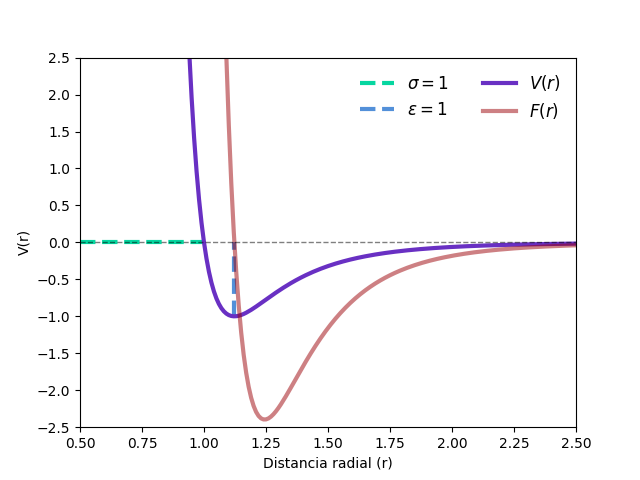
\includegraphics[scale=0.45]{../Graphics/Potencial.png}
    \caption{Potencial y fuerza de Lennard-Jones}
    \label{pot-len-jones}
\end{figure}
Teniendo el potencial de la ecuación \ref{Potencial de Lennard-Jones}, podemos deducir la fuerza, ya que esta puede ser deducida a partir de aplicar el gradiente a la función $V(r)$, teniendo así la siguiente expresión:
\begin{equation}
    \label{eq:fuerzateo}
    \vec{F}(r)= 4\epsilon \left(12\frac{\sigma^{12}}{r^{13}}- 6 \frac{\sigma^6}{r^7} \right) \hat{r}
\end{equation}
reescribiendo las ecuaciones \ref{Potencial de Lennard-Jones} y \ref{eq:fuerzateo} pars tener la suma de estas en un sistema de n particulas se tiene lo siguiente:
\begin{equation}
    \label{eq:pot-n}
    U_t=\left\langle\sum_{i=1}^N \sum_{j<i}^N V_i,j(|r_j-r_i|)\right\rangle_t
\end{equation}
\begin{equation}
    \changefontsizes{9pt}
    \label{eq:f-n}
    F_i = \frac{48}{\sigma^2} \sum_{j \ne i} \left[\left(\frac{\sigma}{r_{ij}}\right)^{14}-\frac{1}{2}\left(\frac{\sigma}{r_{ij}} \right)^8  \right] (r_j-r_i)
\end{equation}
Teniendo ya la dinámica se este sistema podemos ir monitoreando la energía cinética de la siguiente manera:
\begin{equation}
    \label{eq:kin-n}
    T_t=\left\langle \sum_{i=1}^N \frac{1}{2}m|v_i(t)|^2\right\rangle
\end{equation}
por lo tanto, la energía total para un tiempo t será:
\begin{equation}
    \label{eq:e-tot}
    E_t=T_t+U_t
\end{equation}
\section*{Resultados}
Planteando un sistema cuadrangular, en el cual todos los átomos se encuentran alineados como en la figura \ref{pos inicial}.
\begin{figure}[H]
    \hspace*{-0.5cm}
    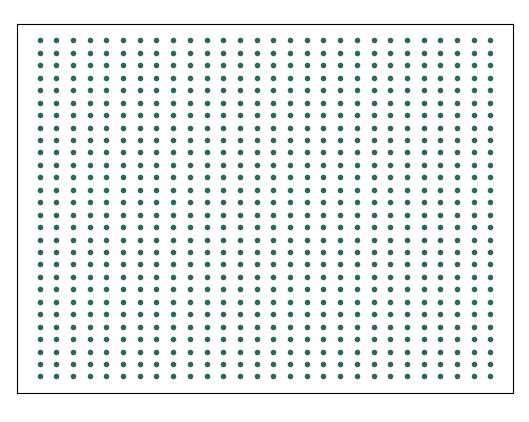
\includegraphics[scale=0.4]{../Graphics/Cor_in.png}\\
    \caption{Posición inicial de la dinámica}
    \label{pos inicial}
\end{figure}
realizando una simulación de la dinámica entre estos átomos realizando 2000000 caminatas con 784 átomos se calculo la distribución radial de la siguiente manera:
\begin{equation}
    \rho(r) = \frac{1}{N} \frac{\left\langle \sum_{i=1}^N n_i(r,\Delta r)  \right\rangle}{\pi r \rho \Delta r}
    \label{eq:rhor}
\end{equation}
donde:
\begin{equation}
    \changefontsizes{11pt}
    \label{eq:area}
    \pi r \Delta r = \pi \left(\left[r +\frac{\Delta r}{2}\right]^2 - \left[r- \frac{\Delta r}{2} \right]^2 \right)
\end{equation}
y la función $n_i(r,\Delta r)$ lleva el conteo del número de átomos que se encuentran en un anillo de radio $r$ y espesor $\Delta r$, llegando así a calcular la función de distribución radial mostrada en la figura \ref{distribución radial}
\begin{figure}[H]
    \centering
    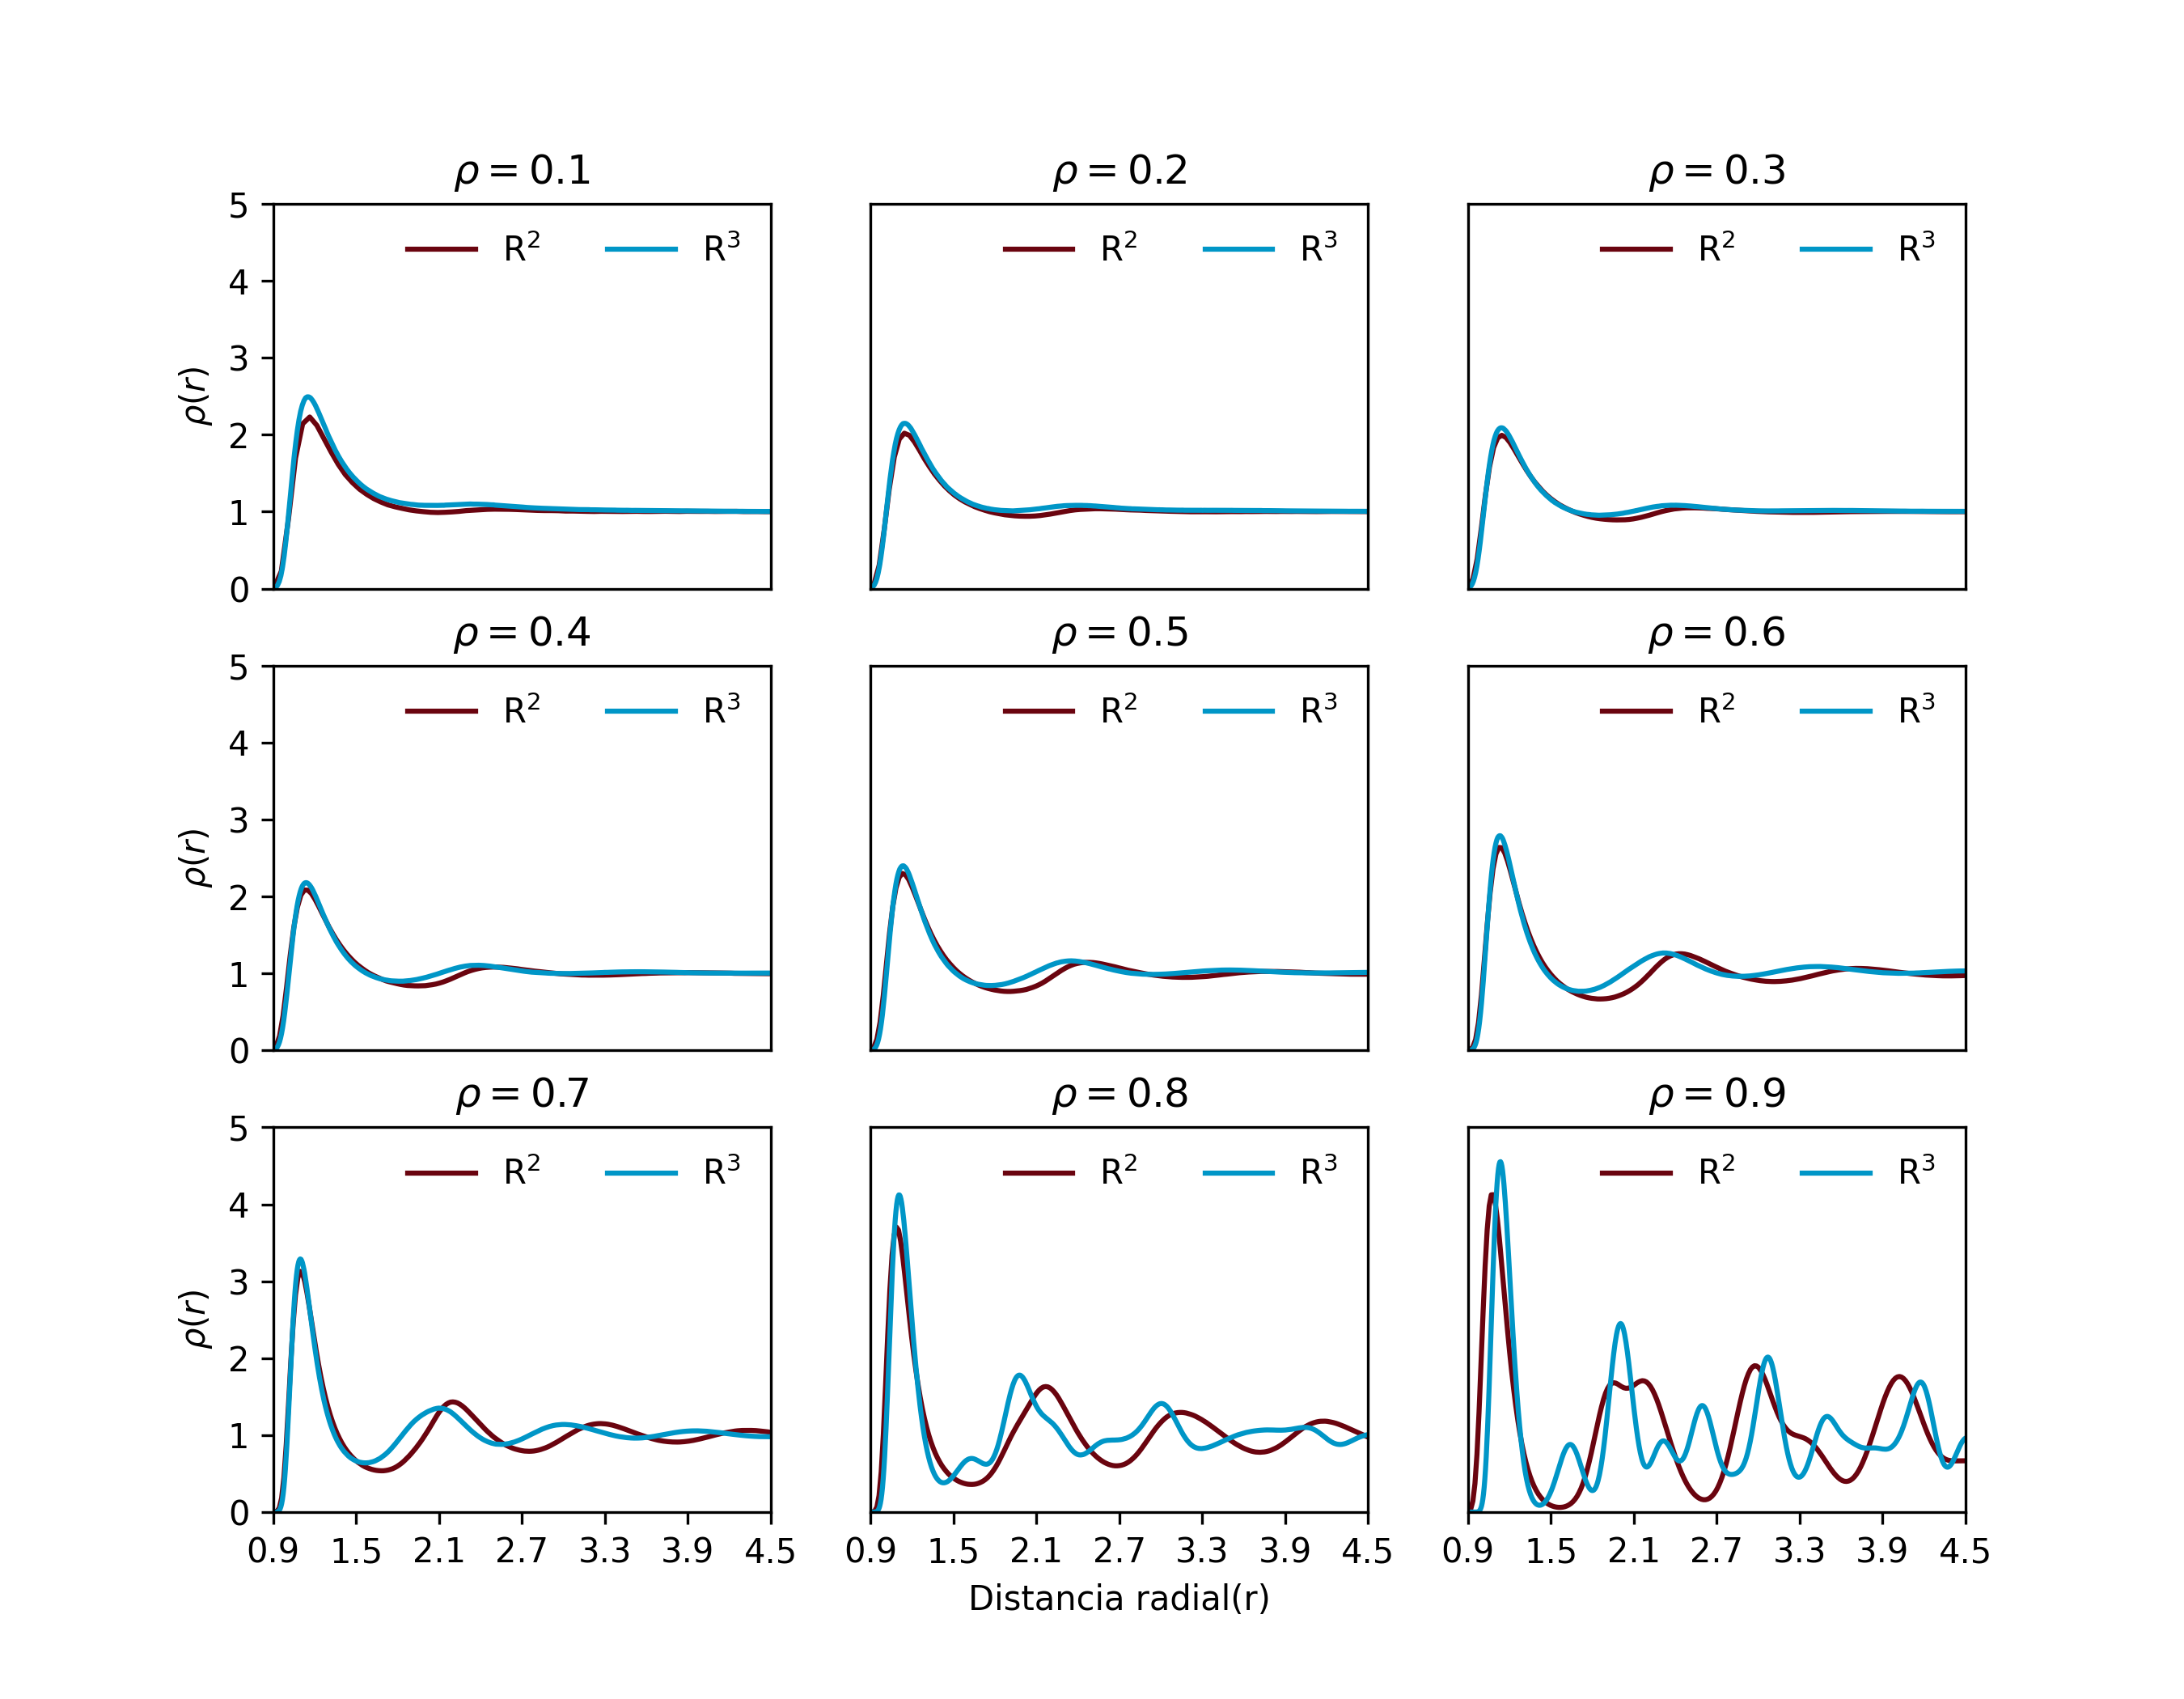
\includegraphics[scale=0.48]{../Graphics/Dis_rad.png}
    \caption{Distribución radial de la estructura}
    \label{distribución radial}
\end{figure}
en la figura \ref{screen dinámica} se observa como es la evolución del sistema conforme se van realizando más pasos en la dinámica. 
La misma simulación lleva acabo el calculo de la energía potencial y la energía cinética conforme las ecuaciones \ref{eq:kin-n} y \ref{eq:pot-n}, por lo que el cálculo de la energía total se realiza de manera simple, con esto en la figura \ref{energias} se muestra la energía cinética, potencial y total del sistema a lo largo de la simulación.
\begin{figure}[H]
    \centering
    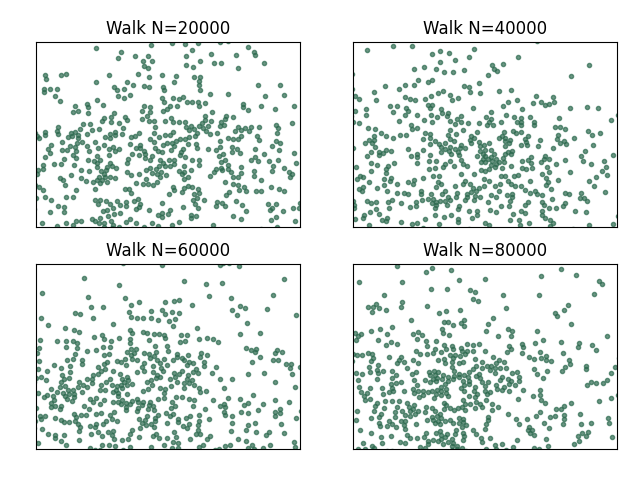
\includegraphics[scale=0.48]{../Graphics/Dim_Graphics.png}
    \caption{Dinámica molecular en diferentes tiempos}
    \label{screen dinámica}
\end{figure}
\begin{figure}[H]
    \hspace{-0.5cm}
    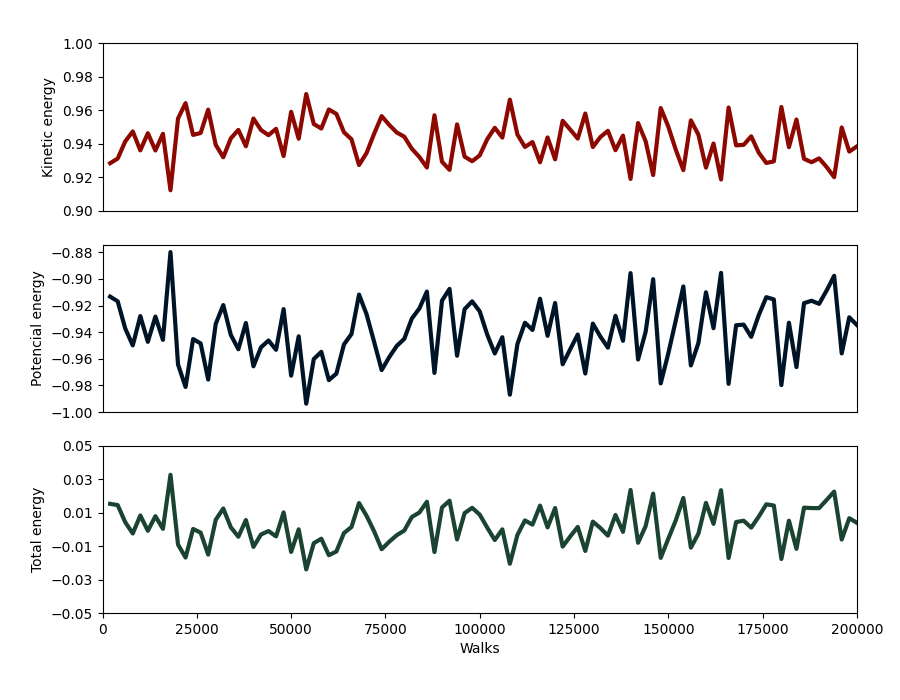
\includegraphics[scale=0.35]{../Graphics/Energy.png}
    \caption{Energía cinética, potencial y total del sistema en toda la simulación}
    \label{energias}
\end{figure}
\section*{Conclusiones}
\section*{Código}
\begin{itemize}
\item \href{https://github.com/giovannilopez9808/Notas_Agosto_2020/blob/master/Simulaciones/Proyecto_1/Scripts/MD-n3.f}{Github - MD-n3.f}\\
Este código contiene la simulación del sistema.
\item \href{https://github.com/giovannilopez9808/Notas_Agosto_2020/blob/master/Simulaciones/Proyecto_1/Scripts/Energy_Graphics.py}{Github - Gráfica de las energías}\\
Este código genera la gráfica \ref{energias}
\item \href{https://github.com/giovannilopez9808/Notas_Agosto_2020/blob/master/Simulaciones/Proyecto_1/Scripts/Cor_Graphics.py}{Github - Gráfica de la posición inicial y Distribución radial}\\
Este código genera la figura \ref{pos inicial} y \ref{distribución radial}
\item \href{https://github.com/giovannilopez9808/Notas_Agosto_2020/blob/master/Simulaciones/Proyecto_1/Scripts/Dim_gif.py}{Github - Animación de la dinámica}\\
Este código genera la animación mostrada en la figura \ref{screen dinámica}
\item \href{https://github.com/giovannilopez9808/Notas_Agosto_2020/blob/master/Simulaciones/Proyecto_1/Scripts/Dim_Graphics.py}{Github - Gráfica para diferentes tiempos}\\
Este código genera la figura \ref{screen dinámica}

\item \href{https://github.com/giovannilopez9808/Notas_Agosto_2020/blob/master/Simulaciones/Proyecto_1/Scripts/Potencial_Graphics.py}{Github - Gráfica del potencial de Lennard-Jones}\\
Este código realiza la figura \ref{pot-len-jones}
\end{itemize}
\bibliographystyle{plain}
\bibliography{Main}
\nocite{*}
\end{multicols}
\end{document}